\section {Раздел ''Безопасность жизнедеятельности``}
\subsection {Синдром компьютерного состояния пользователя}
Анализ синдрома компьютерного состояния пользователя проведён в соответствии с \cite{OFFICESYNDROME, COMPUTERVISION, WRISTPOSTURE, CARPALTUNNEL, SANPIN}.

В настоящее время во многих источниках массовой информации и различных статьях в журналах о здоровье встречается наименование так называемого «компьютерного состояния пользователя». Под ним обычно подразумеваются один или более симптомов, возникающих вследствие продолжительного взаимодействия с СВТ. 

Наиболее широко понятие компьютерного состояния можно рассматривать в рамках «офисного синдрома», включающего в себя заболевания желудочно-кишечного тракта  (гастрит, язва желудка) вследствие неправильного питания, злоупотребления кофе, ожирения вследствие малоподвижного образа жизни, ненормированного рабочего дня, заболевания дыхательной системы, возникающие вследствие используемых в офисных помещениях кондиционеров и потенциально имеющихся там же аллергенов\cite{OFFICESYNDROME}. Самые узкие встречаемые трактовки включают только заболевания органов зрения, вызванные длительными психологическими и физическими нагрузками, в том числе и временные эффекты, появляющиеся из-за усталости после работы, и иногда «туннельный синдром», возникающий вследствие использования компьютерного манипулятора типа «мышь» или «клавиатура». В настоящем разделе под «компьютерным состоянием пользователя» будут пониматься только те эффекты, которые возникают непосредственно в процессе или по причине взаимодействия с компьютерной техникой. Первыми будут рассмотрены симптомы, связанные со зрительной системой.

Основными симптомами, свидетельствующими о проблемах со зрительной системой (или синдром длительных зрительных нагрузок, СДЗН), являются снижение уровня остроты зрения, чувство жжения в глазах, ощущение затуманенности зрения, избыточная светочувствительность, также возможно покраснение глазных яблок и быстрая утомляемость глаз при чтении. Симптомы могут быть выражены более явно, если у человека уже присутствуют те или иные формы зрительных нарушений, как-то: близорукость (миопия), дальнозоркость (гиперметропия) и т.д. Согласно исследованию, среди 795 малазийских студентов, использовавших компьютер более 2х часов ежедневно, те или иные симптомы наблюдались у 90\% опрошенных, причём большую часть жалоб составляла головная боль (19,7\%) и напряжение глаз (16,4\%)\cite{COMPUTERVISION}. При  этом было замечено, что использование зрительных фильтров на мониторах не привело к ослаблению негативных эффектов, а периодические взгляды на удалённые объекты во время работы помогло снизить таковые эффекты. 

Запястный туннельный синдром (или синдром запястного канала пользователя, СЗКП) описывают как последствия работы с клавиатурой, в случае, когда имеет место неправильная эксплуатация ПЭВМ. К симптомам, связанным с запястным туннельным синдромом, обычно относят неприятные ощущения в районе кисти, ладоней или пальцев, последующее ослабление, возможное онемение, опухание, боль или тяжесть кисти целиком, при этом таковые проблемы усиливаются в ночное время. Согласно исследованию, у 20 здоровых людей было проверено влияние различных положений кисти на давление в запястном канале правой руки\cite{WRISTPOSTURE}. Было выявлено значительное влияние угла наклона кисти на давление в запястном канале (максимум наблюдался при 45\degree). Также наблюдалось влияние сгиба локтевого сустава на это давление (максимум наблюдался при 15\degree). При наборе текста давление увеличивалось независимо от положения кисти. Таким образом, для снижения риска развития синдрома запястного канала необходимо использовать эргономичные клавиатуры (возможно, позволяющие разделять стандартную клавиатуру на 2 половины), учитывающие данные наблюдения, а также мебель (стулья, кресла), позволяющие таким образом расположить локти при работе с клавиатурой, чтобы в максимальной степени уменьшить давление в запястном канале. Однако, ряд других исследований  утверждает, что у исследуемой группы лиц пользователей компьютеров не было большей склонности к развитию синдрома запястного канала по сравнению с лицами, не использующими клавиатуру\cite{CARPALTUNNEL}. В действительности, любая профессиональная деятельность, связанная с повышенной вибрацией (перфораторы, отбойные молотки) гораздо чаще служит причиной его развития.

Симптомы, связанные с длительной неподвижностью (или синдром длительных статических нагрузок, СДСН) отдельных частей тела во время работы с компьютером обычно выражаются в болях в нижней части спины, возможно, шее, онемении отдельных областей и/ или пальцев рук или ног. В том числе, возможно появление таких серьёзных заболеваний, как деформация позвоночных дисков.

Синдром нагрузок от излучения компьютера (или синдром длительных нагрузок излучения, СДНИ) может проявляться как в негативном воздействии на зрительную систему, нарушении глазного кровообращения, а в случае использования не соответствующих нормам электронно-лучевых трубок – дозе мягкого рентгеновского излучения более 1 мкЗв/ч\cite{SANPIN}.

Психологические нагрузки, связанные со стрессовыми ситуациями при работе с компьютером (или синдром длительных психологических нагрузок, СДПН) могут возникать по тем же причинам, что и любые стрессовые ситуации в рабочей деятельности. В мире компьютерной техники процветает постоянное появление новых технологий. В конечном счёте, это приводит к тому, что операторам ПЭВМ приходится их изучать, иначе они рискуют остаться за бортом прогресса. Некоторыми пользователями такой вынужденно быстрый темп обучения может восприниматься как психологическое насилие. Большая конкуренция на рынке труда заставляет людей нервничать при каждой совершаемой ошибке при работе с ПК, что в конечном итоге приводит к раздражению, нервным срывам, и, иногда, депрессиям.

\subsection {Мероприятия по снижению компьютерного состояния пользователя}
Мероприятия по снижению компьютерного состояния пользователя разработаны в соответствии с \cite{SANPIN}.

Для снижения компьютерного состояния пользователя большое значение имеет правильная организация рабочего места. Схема размещения рабочего места пользователя представлена на рисунке \ref {fig:workplace}. Для работы за компьютером человек располагается на рабочем месте указанным образом. Все обозначения на схеме представлены в сантиметрах. 

\begin {figure}[h]
	\centering
	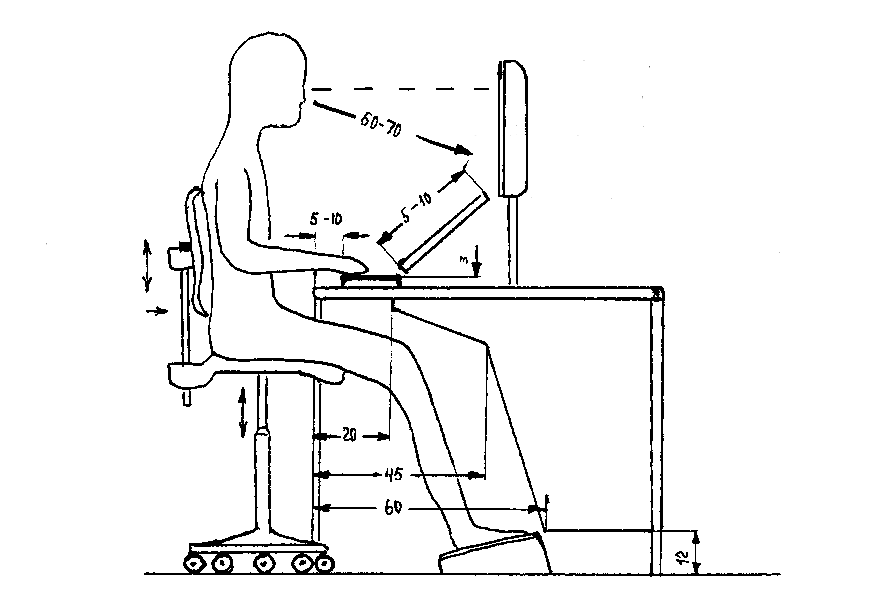
\includegraphics[scale=0.9]{img/WorkPlace.png}
	\caption{Схема рабочего места пользователя}
	\label{fig:workplace}
\end {figure}

Рекомендованная для снижения синдрома запястного канала пользователя и синдрома длительных статических нагрузок деятельность подразумевает \cite{SANPIN}:
\begin {enumerate}
	\item Расстояние от видеомонитора до глаз человека составляет около 600-700 мм, в крайнем случае, 500 мм при чтении слишком мелкого шрифта. При этом присутствует возможность регулировки по высоте поверхности, на которой установлен монитор, в пределах 460-520 мм при глубине не менее 550 мм и ширине более 600 мм.
	\item Стол для работы с ПЭВМ имеет определённую высоту в зависимости от роста пользователя. Также имеется соответствующее пространство для ног. Указанная зависимость размещена в таблице \ref{table:tableheight}.
	\item Рабочий стул предоставляет возможность регулировать наклон спинки и сидения, имеет подъёмно-поворотный механизм, при этом его параметры зависят от высоты пользователя. Указанная зависимость размещена в таблице \ref{table:chairheight}.
	\item Расстояние между соседними рабочими местами в направлении, перпендикулярном экрану монитора, составляет не менее 2,0 м, а между боковыми поверхностями – 1,2 м.
\end {enumerate}
\begin{table}[t]
	\begin {tabular}{|p{10em}|p{10em}|p{10em}|}
		\hline
		Рост пользователя в обуви, см & \multicolumn{2}{|p{20em}|}{Высота над полом, см}\\ \cline{2-3}
                      & поверхность стола & пространство для ног, не менее\\ \hline
		116---130 & 52 & 40\\ \hline
		131---145 & 58 & 52\\ \hline
		146---160 & 64 & 58\\ \hline
		161---175 & 70 & 64\\ \hline
		выше 175 & 76 & 70\\ \hline
	\multicolumn{3}{|p{30em}|}{Примечание: ширина и глубина пространства для ног определяются конструкцией стола.}\\ \hline
	\end {tabular}
	\caption{Высота одноместного стола для занятий с персональным компьютером}
	\label{table:tableheight}
\end{table}

\begin{table}[t]
	\begin {tabular}{|p{15em}|p{3em}|p{3em}|p{3em}|p{3em}|p{3em}|}
		\hline
		Параметры стула & \multicolumn{5}{|p{15em}|}{Рост пользователя в обуви, см}\\ \cline{2-6}
		& 116 --- 130 & 131 --- 145 & 146 --- 160 & 161 --- 175 & >175 \\ \hline
                      Высота сиденья над полом, мм & 300 & 340 & 380 & 420 & 460\\ \hline
		Ширина сиденья, не менее, мм & 270 & 290 & 320 & 340 & 360\\ \hline
		Глубина сиденья, мм & 290 & 330 & 360 & 380 & 400\\ \hline
		Высота нижнего края спинки над сиденьем, мм & 130 & 150 & 160 & 170 & 190\\ \hline
		Высота верхнего края спинки над сиденьем, мм & 280 & 310 & 330 & 360 & 400\\ \hline
		Высота линии прогиба спинки, не менее, мм & 170 & 190 & 200 & 210 & 220\\ \hline
		Радиус изгиба переднего края сиденья, мм & \multicolumn{5}{|p{18em}|}{20 --- 50}\\ \hline
		Угол наклона сиденья, \degree & \multicolumn{5}{|p{18em}|}{0 --- 4}\\ \hline
		Угол наклона спинки, \degree & \multicolumn{5}{|p{18em}|}{95 --- 108}\\ \hline
		Радиус спинки в плане, не менее, мм & \multicolumn{5}{|p{18em}|}{300}\\ \hline
	\end {tabular}
	\caption{Параметры стула для работы с ПЭВМ в зависимости от роста пользователя}
	\label{table:chairheight}
\end{table}
Рекомендованный комплекс зрительных упражнений имеет несколько вариантов, которые необходимо регулярно чередовать при использовании \cite{SANPIN}.

Первый вариант:
\begin {enumerate}
	\item Закрыть глаза, не напрягая  глазные мышцы, на счёт 1 --- 4; широко раскрыть глаза и посмотреть вдаль на счёт 1 --- 6; повторить до 5 раз.
	\item Посмотреть на кончик носа на счёт 1 --- 4, а потом перевести взгляд вдаль на счёт 1 --- 6; повторить до 5 раз.
	\item Не поворачивая головы (держа прямо), делать медленно круговые движения глазами вверх-вправо-вниз-влево и в обратную сторону.
	\item При неподвижной голове перевести взор с фиксацией его на счёт 1 --- 4 вверх, на счёт 1 --- 6 прямо; после этого аналогичным образом вниз-прямо, вправо-прямо, влево-прямо; проделать движение по диагонали в одну и другую сторону с переводом глаз прямо на счёт 1 --- 6; повторить до 4 раз.
\end {enumerate}

Второй вариант:
\begin {enumerate}
	\item Голову держать прямо; поморгать, не напрягая глазные мышцы, на счёт 1 --- 15.
	\item Не поворачивая головы (держа прямо) с закрытыми глазами, посмотреть вправо на счёт 1 ---  4 , затем налево на счёт 1 --- 4 и прямо на счёт 1 --- 6; повторить до 5 раз.
	\item Посмотреть на указательный палец, удалённый от глаз на расстояние 25-30 см, на счёт 1 --- 4, потом перевести взор вдаль на счёт 1 --- 6; повторить до 5 раз.
	\item В среднем темпе проделать 3 --- 4 круговых движения глазами в правую сторону, столько же в левую сторону, и, расслабив глазные мышцы, посмотреть вдаль на счёт 1 --- 6; повторить до 2х раз.
\end {enumerate}

Ограничение на работу с ЭВМ накладывается в зависимости от вида и категории трудовой деятельности. При работе с ПК обычно выделяют три категории деятельности. К группе А относят считывание информации с видеодисплея с предварительным запросом. К группе Б относят работу по вводу информации. Группа В означает творческую работу в интерактивном режиме с ПЭВМ. Если человек выполняет работу, попадающую сразу в несколько из указанных групп, следует считать, что у него та группа, работа в которой занимает более половины рабочего времени. 

Для этих групп устанавливаются категории тяжести, причём по нагрузке предельными для группы А является считывание до 60000 знаков за смену, по группе Б --- не более 40000 знаков за смену, для группы В --- не более 6 рабочих часов за смену \cite{SANPIN}.

В зависимости от описанных категорий тяжести и группы трудовой деятельности устанавливается суммарное время регламентированных перерывов, указанное в таблице \ref{table:workbreaks}.
\begin{table}[h]
	\begin {tabular}{|p{5em}|p{5em}|p{5em}|p{4em}|p{3em}|p{6em}|}
		\hline
		Категория работы с ПЭВМ & \multicolumn{3}{|p{14em}|}{Уровень нагрузки за рабочую смену при видах работ с ПЭВМ} & \multicolumn{2}{|p{9em}|}{Суммарное время регламентированных перерывов, мин}\\ \cline{2-6}
		& группа А, количество знаков & группа Б, количество знаков & группа В, ч & при 8-часовой смене & при 12-часовой смене \\ \hline
                     I & до 20 000 & до 15 000 & до 2 & 50 & 80\\ \hline
		II & до 40 000 & до 30 000 & до 4 & 70 & 110\\ \hline
		III & до 60 000 & до 40 000 & до 6 & 90 & 140\\ \hline
	\end {tabular}
	\caption{Суммарное время регламентированных перерывов в зависимости от различных факторов при работе с ПЭВМ}
	\label{table:workbreaks}
\end{table}

В любом случае, продолжительность непрерывной работы не должна превышать одного часа. Если работа осуществляется в ночное время, продолжительность указанных перерывов считают увеличенной на 30\%. Если при соблюдении указанных норм всё равно проявляются симптомы зрительного напряжения, осуществляется разработка индивидуального плана по работе с ПК \cite{SANPIN}. Если тот или иной симптом принимает острые формы – немедленно обратиться к офтальмологу.

\subsection {Экологическая оценка и технологическая схема переработки компьютерного лома}
Экологическая оценка и технологическая схема переработки компьютерного лома проведена в соответствии с \cite {EWASTE, SNIP, ECOLOGY}.

На рисунке \ref{fig:garbageflow} приведена технологическая схема переработки компьютерного лома, применяемая в одной из ведущих фирм Австралии в данной области E-Waste \cite {EWASTE}. 
\begin {figure}[h!]
	\centering
	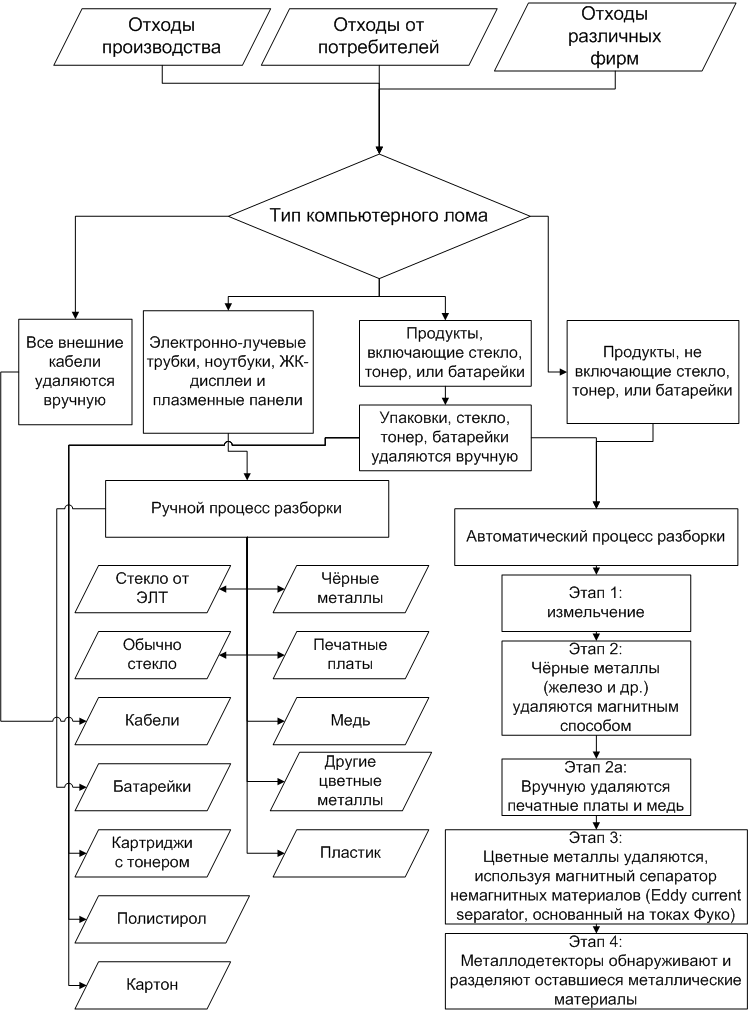
\includegraphics[scale=0.6]{img/ComputerGarbage.png}
	\caption{Технологическая схема переработки компьютерного лома}
	\label{fig:garbageflow}
\end {figure}

Несмотря на большое количество заявленных в схеме ручных процессов, а также тот фактор, что фирма позиционирует себя с точки зрения отказа от использования свалочных полигонов, E-Waste существует более 5 лет (2011-2016), что свидетельствует о потенциальной возможности масштабирования данной технологической схемы переработки. В печатных материалах говорится о потенциальной возможности восстановлении до 95-98 \% использованных при создании техники исходных материалов.

С точки зрения соответствия экологическим нормам применяемых в сконструированной схеме технологических процессов, разделение на потоки различных типов лома и большое количество ручного труда позволяют избежать многих экологически вредных процедур, последующего сжигания и отправку лома на свалку, где при захоронении уже невосстановимых отходов пришлось бы руководствоваться нормами \cite{SNIP}. Используемые магнитные техники восстановления металлов позволяют избежать нагрева и возможного плавления присутствующих в смеси отходов полимерных материалов, которые при горении выделяют различные токсичные вещества (в зависимости от состава пластмассы – даже яды, как стирол, диоксины и т.д.).

Применение такой схемы может быть связано со следующими особенностями \cite {ECOLOGY}:

\begin {enumerate}
	\item В состав системного блока ПЭВМ входит примерно 20.5 \% железа, 14.2 \% алюминия, 6.3 \% свинца, 0,0189 \% серебра и 0,016 \% золота, а также другие металлы. Поскольку процент драгоценных металлов так невелик, для поддержания рентабельности деятельности по переработке компьютерных отходов необходимо обеспечивать значительную эффективность восстановления материала. Другие существующие технологические процессы, основанные на использовании различных химических реакций, могут давать большую эффективность. Поэтому переход на более экологически чистую и менее экономически выгодную схему не выглядит таким привлекательным, даже учитывая тот факт, что химическая обработка требует специальной схемы для каждого отдельного типа металла. Например, содержащие платину отходы вначале помещаются в ванну с расплавленным алюминием, затем – в 15 \% раствор кипящей серной кислоты в течение 5 часов, в итоге получая концентрат, содержащий более 90 \% металла. Серебряный лом перед переработкой требует хлорирования в течение порядка 3 часов, но это обеспечивает эффективность извлечения порядка 99,5 \%. Для золота могут использовать выщелачивание в диафрагменном охлаждаемом электролизере, в итоге дающем выход до 99,8 \% содержимого. Всё же, осуществление набора всех основанных на химических реакциях процессов в рамках одного производства требует тщательного контроля соблюдения техники безопасности и экологических норм по выбросам отходов, поэтому, по крайней мере, с этой точки зрения магнитная схема извлечения металлов выглядит проще и безопаснее.
	\item Такой подход требует раздельной утилизации компьютерной техники и остальных отходов. Несмотря на то, что в отдельных регионах нашей страны уже производятся попытки привить культуру раздельной утилизации, в большинстве своём даже при желании раздельно утилизировать отходы попросту нет возможности. Единственная возможность для обычного гражданина избежать отправки на свалку устаревшей и/или повреждённой компьютерной техники – сдать/продать кому-то лично или на запчасти в ремонтные фирмы.
\end {enumerate}
